\documentclass[norsk,a4paper,12pt]{article}
\usepackage[T1]{fontenc} %for å bruke æøå
\usepackage[utf8]{inputenc}
\usepackage{graphicx} %for å inkludere grafikk
\usepackage{verbatim} %for å inkludere filer med tegn LaTeX ikke liker
\usepackage{amsfonts}
%\usepackage[framed]{mcode} %for å få inn matlabkode
\usepackage{listings}
\usepackage[margin=1.2cm]{caption} % skalere figur text
\usepackage{subfigure}

\bibliographystyle{plain}
\usepackage{parskip}
\usepackage{babel, textcomp, color, amsmath, amssymb, tikz, subfig, float}
\renewcommand{\captionfont}{\sffamily\small} 
\renewcommand{\captionlabelfont}{\bf} 
\fboxsep=0mm % ramme inn bilder


\title{FYS3150 - Project 4}
\author{Steffen Brask}
\date{\today}


\begin{document}

\maketitle

\begin{center}
https://github.com/steffemb/project4/tree/master/Levering
\end{center}


\newpage


\section*{Abstract}

In this project we will test the numerical stability of thre different algorithms for solving differential equations.

\section*{Introduction}

In this project we are going to test the stability and errors of thre methods for solving partial differential equations.
We will write a program that solves the diffusion equation with the explicit and implicit Euler scheme, and last the Crank Nichols scheme.

the equation to solve is:

\begin{equation}
 \frac{\partial u(x,t)}{\partial x^2} = \frac{\partial u(x,t)}{\partial t}
\end{equation}

with initial conditions $u(x,0) = 0, 0<x<d$, and $u(0,t) = 1, t>0$, and $u(d,t) = 0, t>0$


\section*{Solution}

First we write a code for the explicit Euler scheme. Mathematically this is written:

\begin{equation}
 \frac{u(x_i,t_j+\Delta t)-u(x_i,t_j)}{\Delta t} = \frac{u(x_i+\Delta x,t_j)-2u(x_i,t_j)+u(x_i-\Delta x,t_j)}{\Delta x^2}.
\end{equation}

This is fairly easy to write an algorithm for, we only need to solve for $t_j + \Delta t$, and we get the equation:

\begin{equation}
 u(x_i,t_j+\Delta t) = u(x_i,t_j) + \frac{\Delta t}{\Delta x^2} u(x_i+\Delta x,t_j)-2u(x_i,t_j)+u(x_i-\Delta x,t_j).
\end{equation}

The algoritm now only needs a for loop over j, and i, which is the time and space indexes. Note that the i indexes must exlude
the first and last indexes.

The second task is to implement the Implicit Euler scheme. We startwith the mathematical expression:

\begin{equation}
 \frac{u(x_i,t_j)-u(x_i,t_j-\Delta t)}{\Delta t} = \frac{u(x_i+\Delta x,t_j)-2u(x_i,t_j)+u(x_i-\Delta x,t_j)}{\Delta x^2}.
\end{equation}

This time we solve for $t_j - \Delta t$, and we get:

\begin{equation}
 u(x_i,t_j-\Delta t) = u(x_i,t_j) - \frac{\Delta t}{\Delta x^2} u(x_i+\Delta x,t_j)-2u(x_i,t_j)+u(x_i-\Delta x,t_j)
\end{equation}

Lets define $\alpha = \frac{\Delta t}{\Delta x^2}$. And rewrite the equation as a linear equation.

\begin{equation}
 u(x_i,t_j-\Delta t) = u(x_i,t_j) -\alpha \hat A u(x_i,t_j),
\end{equation}

where $\hat A$ is the matrix:

\begin{equation}
    {\bf A} = \left(\begin{array}{cccccc}
                           -2& 1& 0 &\dots   & \dots &0 \\
                           1 & -2 & 1 &0 &\dots &\dots \\
                           0&1 &-2 & 1 & 0 & \dots \\
                           & \dots   & \dots &\dots   &\dots & \dots \\
                           0&\dots   &  &1 &-2& 1 \\
                           0&\dots    &  & 0  &1 & -2 \\
                      \end{array} \right)
\end{equation}

further:

\begin{equation}
 u(x_i,t_j-\Delta t) = u(x_i,t_j)(\hat I -\alpha \hat A),
\end{equation}

And we can define:

\begin{equation}
 \hat B = (\hat I -\alpha \hat A)
\end{equation}


\begin{equation}
    {\bf B} = \left(\begin{array}{cccccc}
                           1+2\alpha& -\alpha& 0 &\dots   & \dots &0 \\
                           -\alpha & 1+2\alpha & -\alpha &0 &\dots &\dots \\
                           0&-\alpha &1+2\alpha & -\alpha & 0 & \dots \\
                           & \dots   & \dots &\dots   &\dots & \dots \\
                           0&\dots   &  &-\alpha &1+2\alpha& -\alpha \\
                           0&\dots    &  & 0  &-\alpha & 1+2\alpha \\
                      \end{array} \right)
\end{equation}

Now scince $\hat B = \hat B^{-1}$, $ u(x_i,t_j) = \hat B u(x_i,t_j-\Delta t)$. This we can solve with a forward and backward substitution.
For details see project 1.

The last task is to implement the Crank Nichols scheme. We can here also start with the mathematical expression:


\begin{equation}
\begin{split}
 \frac{u(x_i,t_j+\Delta t)-u(x_i,t_j)}{\Delta t} = \frac{1}{2}\left(\frac{u(x_i+\Delta x,t_j)-2u(x_i,t_j)+u(x_i-\Delta x,t_j)}{\Delta x^2}+\right. \\
 \left. \frac{u(x_i+\Delta x,t_j+\Delta t)-2u(x_i,t_j+\Delta t)+u(x_i-\Delta x,t_j+\Delta t)}{\Delta x^2} \right).
 \end{split}
\end{equation}

This expression can be a bit misleading. If we stare a bit at this equation we see that there are two parts that look the same as 
in the two schemes above. What isn't clear in eq. 10 is that we wish to solve with the explicit scheme first and the use tis solution
in the implicit. It really is as easy as that but let me clarify a couple of details first. We rewrite the equation: 

\begin{equation}
\begin{split}
 2(u(x_i,t_j+\Delta t)-u(x_i,t_j)) = \alpha\left( (u(x_i+\Delta x,t_j)-2u(x_i,t_j)+u(x_i-\Delta x,t_j)) +\right. \\
 \left. (u(x_i+\Delta x,t_j+\Delta t)-2u(x_i,t_j+\Delta t)+u(x_i-\Delta x,t_j+\Delta t)) \right).
 \end{split}
\end{equation}

We see that we get a factor of two which changes our $\hat B$ matrix, so $ \hat B' = (2 \hat I -\alpha \hat A)$

and the algoritm is now simply:

solve u(x,t) with explicit scheme.

put these u(x,t) values into the implicit sceme and solve using the $\hat B'$ matrix.

put u(0,t) += alpha

The last point is a cool trick to let us solve for u staigt away without changing to ``simpler'' boundary conditions.
This comes from the first row of matrix $\hat B'$. In project 1 we had a matrix with two fictive points in the begining and end
that where 0. So they gave us no problems. Now the points are $-\alpha$. if we write out the equation it gieldes, it goes as follows:


\begin{equation}
 -\alpha u_0 + (2+2\alpha) u_1 - \alpha u_2 = u_1 \Rightarrow (2+2\alpha) u_1 - \alpha u_2 = u_1 + \alpha
\end{equation}

So we simply add $\alpha$ to the first entry.

\section*{Results}

It is hard to get good results when i havent managed to find the closed form solution. My final expression tok form:

\begin{equation}
 \sum_{n=1}  \frac{(-1)^{n+1}}{n \pi} sin(\frac{\pi x}{L}) \sum_{k=0} \frac{(\frac{-n^2 \pi^2 t}{L})^k}{k!}
\end{equation}

But i did not manage to get rid of the sumations. So instead of error analysis i wil mainly speak about stability.

\begin{figure}[H]
  \begin{center}
    \subfigure[explicit, dt = 0,006]{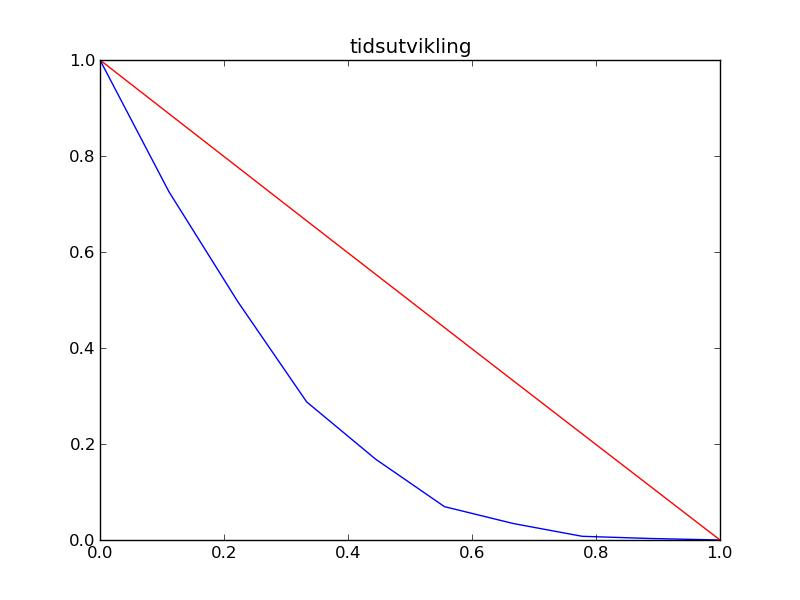
\includegraphics[scale=0.2]{stable_explicit_dt_0,006.jpg}}
    \subfigure[implicit, dt = 0,006]{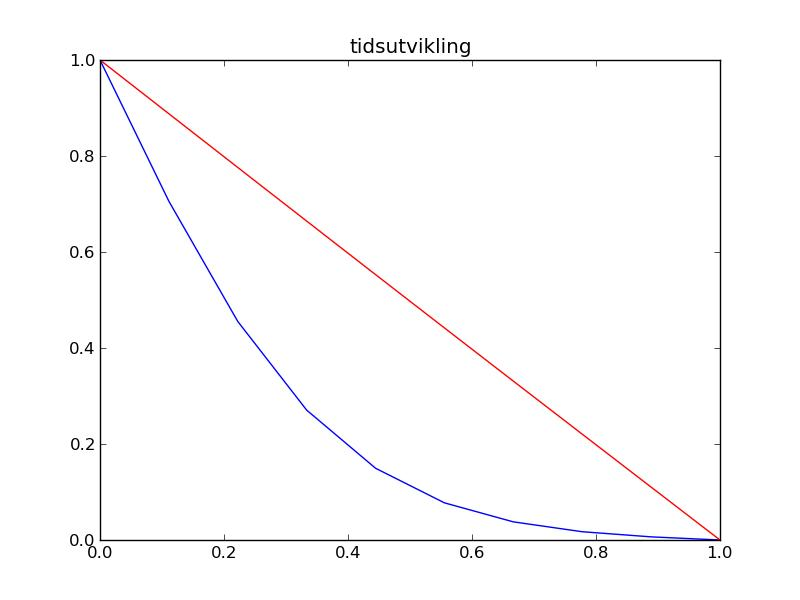
\includegraphics[scale=0.2]{stable_implicit_dt_0,006.jpg}}
    \subfigure[crank nichols, dt = 0,006]{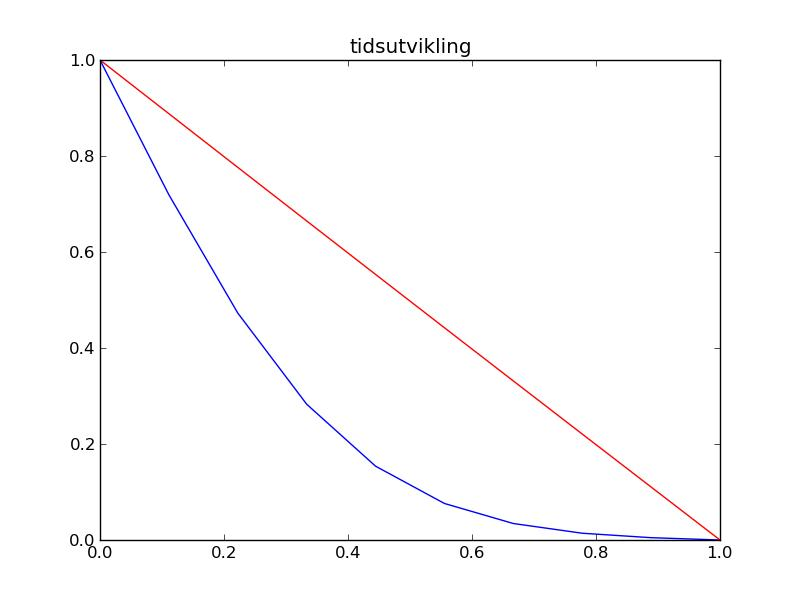
\includegraphics[scale=0.2]{stable_crank_dt_0,006.jpg}}
    \subfigure[explicit, dt = 0,01]{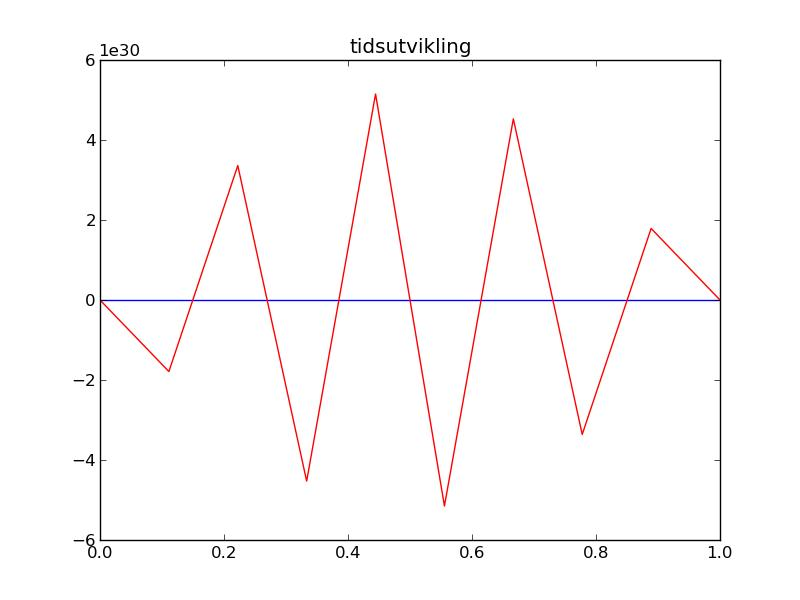
\includegraphics[scale=0.2]{unstable_explicit_dt_0,01.jpg}}
  \end{center}
 \caption{\textit{Plot of solutions with the different schemes}}
  \label{fig:edge}
\end{figure}

These plots are mostly interesting seen against the truncation errors, which i don't have. But We see that for the explicit scheme 
we lose stability at dt = 0,01, in general stability is lost if $\alpha < \frac{1}{2}$. In contrast to the implicit scheme that seemed
to never loose stability, although the error will probably be way over axeptable values for large dt's.

The Crank Nichols Scheme is somewhere in between. I lost stability at dt = 0.04


\section*{Conclusion}

It's hard to conclude with annything out from these humble results. I am guessing that the Crank Nichols scheme has the best
truncation error, and will therefore be the algorithm of choise. It is important to note though that it is also the heaviest algorithm
by far, scince we basically do both the other algorithms calculations in it. In the case where we need stability over error, the 
implicit scheme will be best. The implicit scheme seems to always give a reasonable solution. So if we only need to see ``how''
the system evolves this will always give us a satisfactory solution. The explicit scheme is the lightest, and therefore it might 
be the best choise if we are doing large computations.


%\subsection*{}

%\begin{figure}[H]
%  \begin{center}
%    \subfigure[N = 10]{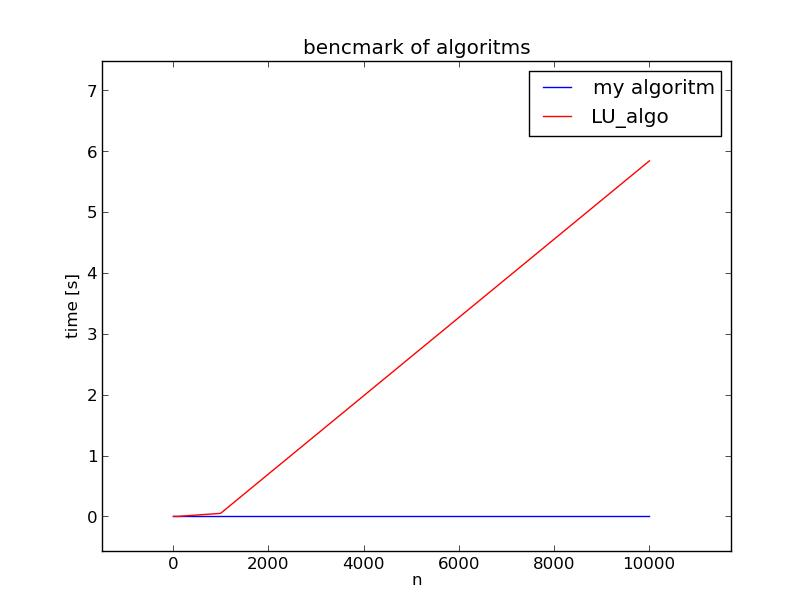
\includegraphics[scale=0.5]{benchmark.jpg}}
%  \end{center}
% \caption{\textit{plot benchmark times for the two different methods of solving}}
%  \label{fig:edge}
%\end{figure}

 
%\newpage

%\section*{Attachments}

%\textbf{Attachment 1: C++ main program}\newline

%\lstinputlisting[language=C++]{main.cpp}

%\newpage

\end{document}








